
\documentclass[12pt,t]{beamer}
\usepackage[utf8]{inputenc}
\usepackage{graphicx}
%\usepackage{amssymb,amsmath}
%\usepackage{verbatim} 
%\usepackage{url}
%\usepackage{float}
%\usepackage{color}
%\usepackage{listings}
%\usepackage{hyperref}
%\usepackage{subfig}
\usepackage{pslatex}
\usetheme[unit=ics,dk]{Frederiksberg}
\title{Detektion af vesikler i celler}
\subtitle{Bachelorforsvar}
\author{Claes Nøhr Ladefoged \and \\
Marcus Bjerg Gregersen}
\institute{Datalogisk Institut}
\date[]{20. Juni 2011}
\begin{document}
\frame[plain]{\titlepage}
\begin{frame}
\frametitle{Resultatet}
\begin{figure}[H]
	\centering
	\begin{minipage}[b]{0.49\linewidth}
		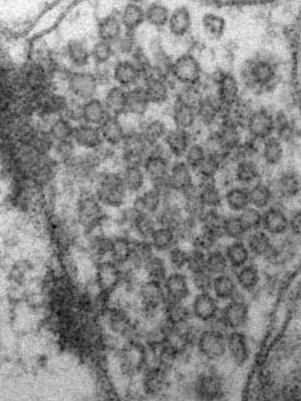
\includegraphics[scale=0.4]{img/ves/0.jpg}
	\end{minipage}
	%\hspace{0.5cm}
	\begin{minipage}[b]{0.49\linewidth}
		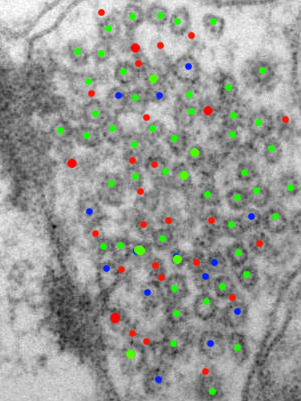
\includegraphics[scale=0.4]{img/ves/1_2.png}
	\end{minipage}
\end{figure}
\end{frame}

\begin{frame}
\frametitle{Introduktion}
\begin{figure}[H]
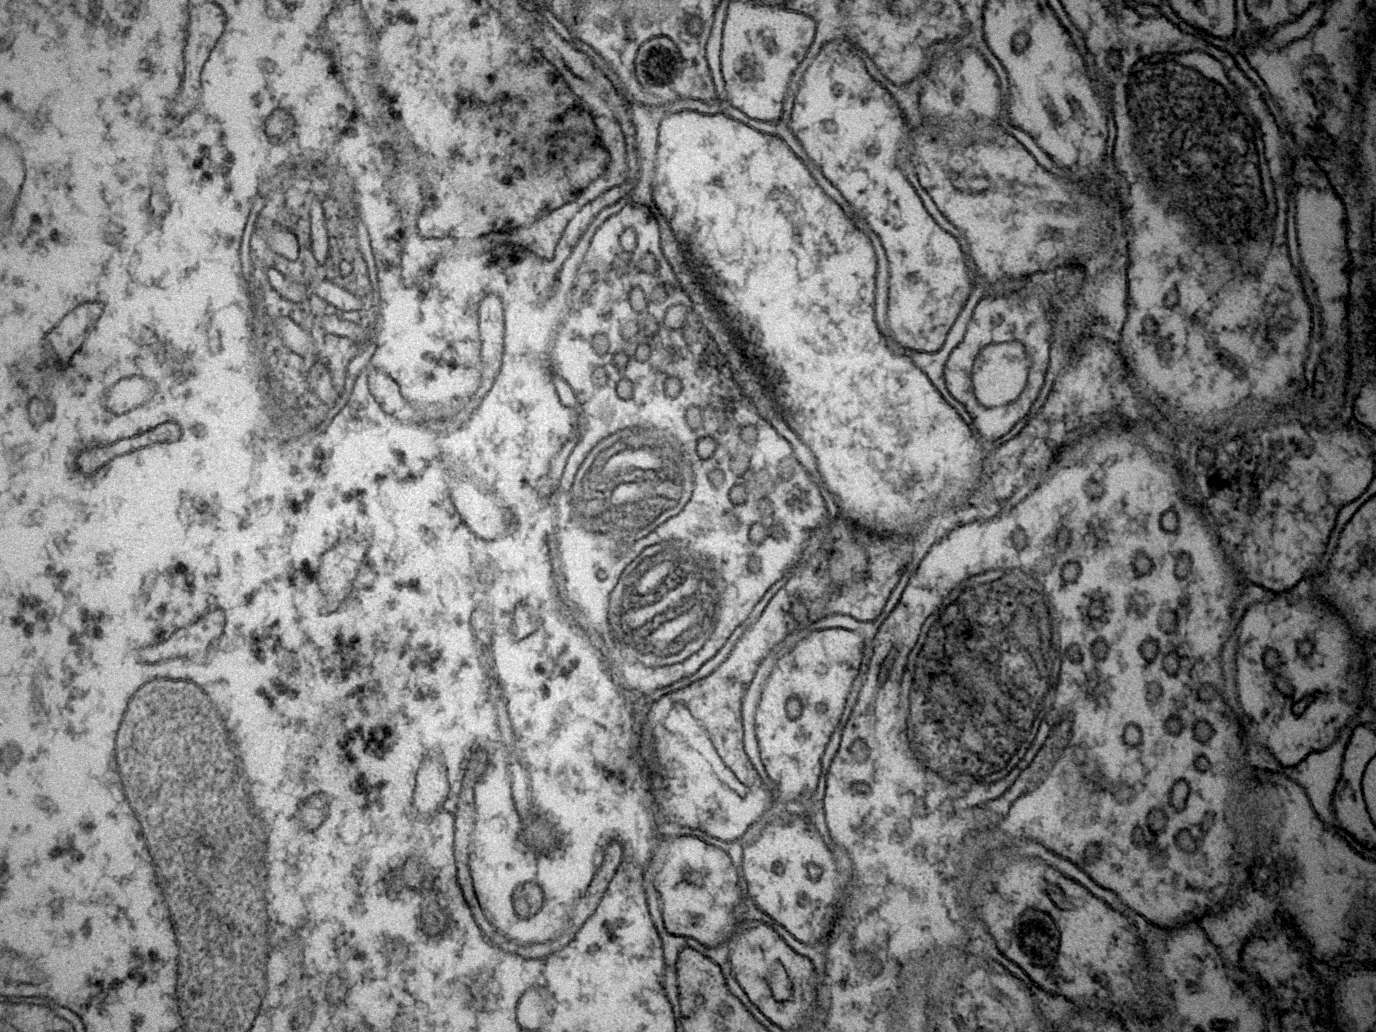
\includegraphics[scale=0.4]{img/orig/AN2-3_7.jpg}
\end{figure}
\end{frame}

\begin{frame}
\frametitle{Introduktion}
\begin{figure}[H]
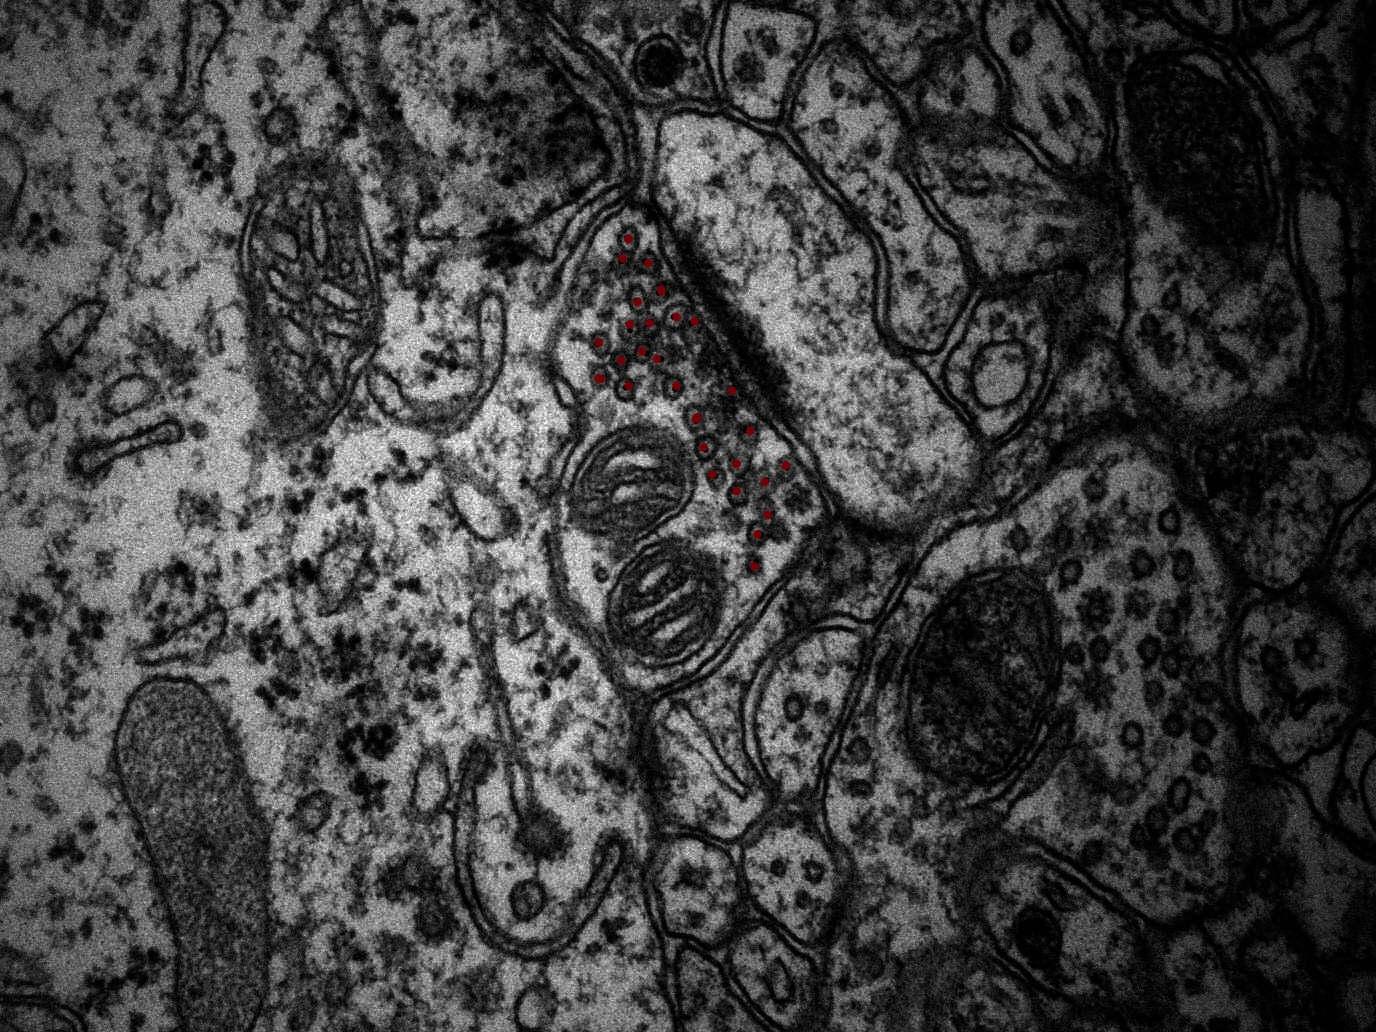
\includegraphics[scale=0.4]{img/orig/AN2-3_7_new.jpg}
\end{figure}
\end{frame}

\begin{frame}
\frametitle{Mesh af en vesikel}
\begin{figure}[H]
	\centering
	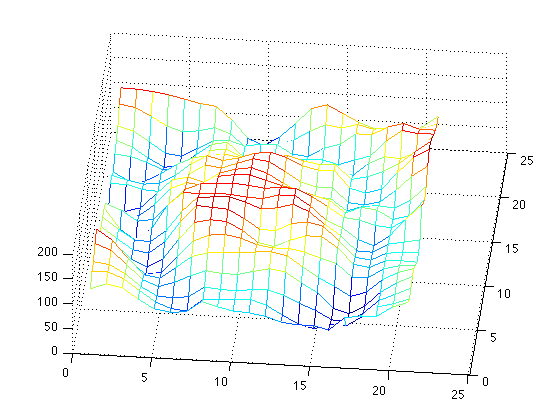
\includegraphics[scale=0.4]{img/ves/mesh.png}
\end{figure}
\end{frame}

\begin{frame}
\frametitle{Billedbehandling - Fouriertransformation \& foldning}
Fouriertransformation
\begin{align*}
	F\{f(u)\} &= \int_{-\infty}^{\infty} f(x) e^{-2 \pi i u x} dx
\end{align*}

Foldning
\begin{align*}
	f(t)*g(t)=\int_{-\infty}^{\infty}f(\tau)g(t-\tau)d\tau
\end{align*}
Relation
\begin{align*}
	f(t)*g(t)= F^{-1} \{F\{f\} \cdot  F\{g\} \}
\end{align*} 

\end{frame}


\begin{frame}
\frametitle{Billedbehandling - Fouriertransformation}
\begin{figure}[H]
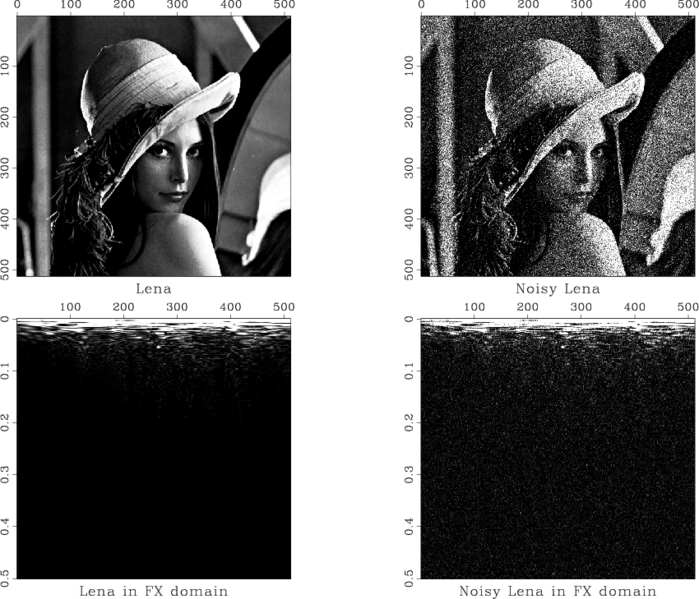
\includegraphics[scale=0.33]{img/billedbeh/lenaex.png}
\end{figure}
\end{frame}

\begin{frame}
\frametitle{Billedbehandling - Fouriertransformation}
\begin{figure}[H]
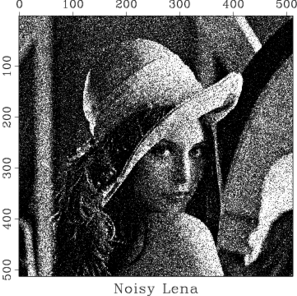
\includegraphics[scale=0.29]{img/billedbeh/lenaex3.png}
\end{figure}
\begin{figure}[H]
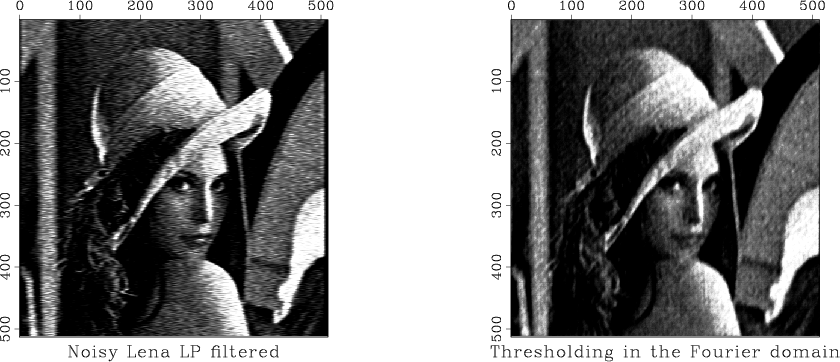
\includegraphics[scale=0.29]{img/billedbeh/lenaex1.png}
\end{figure}
\end{frame}

% \begin{frame}
% \frametitle{Billedbehandling - Foldning}
% %Foldning opnås ved
% \begin{align*}
% 	f(t)*g(t)=\int_{-\infty}^{\infty}f(\tau)g(t-\tau)d\tau
% \end{align*}
% %hvor $*$ er tegnet for foldning. 
% 
% \end{frame}

\begin{frame}
\frametitle{Billedbehandling - Gaussisk udglatning}
\begin{align*}
	G(x,y) = \frac{1}{2\pi\sigma^2}e^{-\frac{x^2+y^2}{2\sigma^2}}\label{ali:premethod_gaussG}
\end{align*}

\begin{figure}[H]
	\centering
	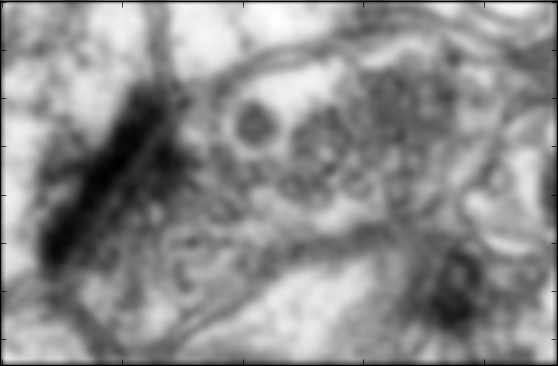
\includegraphics[scale=0.5]{../files/premethod/img/gausscell.png}
\end{figure}
\end{frame}

\begin{frame}
\frametitle{Billedbehandling - Sobelfilter}
\begin{align*}
	G_y = \begin{bmatrix}
		-1 & -2 & -1\\
		0 & 0 & 0\\
		1 & 2 & 1
	\end{bmatrix} * I
	&&
	G_x = \begin{bmatrix}
		-1 & 0 & 1\\
		-2 & 0 & 2\\
		-1 & 0 & 1
	\end{bmatrix} * I
	\end{align*}
\begin{align*}
	G &= \sqrt{G_x^2 + G_y^2}
	&\Theta = \arctan\left(\frac{G_y}{G_x}\right)
\end{align*}
\end{frame}

\begin{frame}
\frametitle{Billedbehandling - Sobelfilter}
\begin{figure}[H]
	\centering
	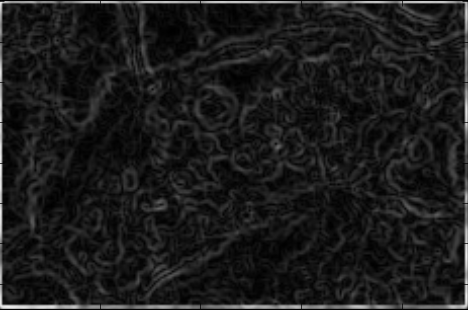
\includegraphics[scale=0.4]{../files/premethod/img/sobel3.png}
\end{figure}
\begin{figure}[H]
	\centering
	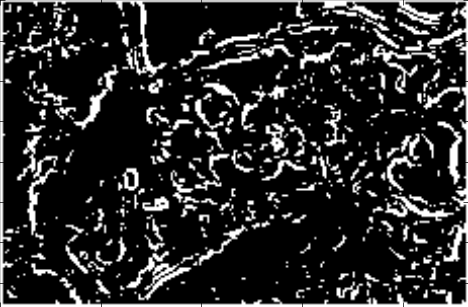
\includegraphics[scale=0.4]{../files/premethod/img/edgemap2.png}
\end{figure}
\end{frame}

Tester


\begin{frame}
\frametitle{Segmentering med eksempelbilleder}
\begin{figure}[H]
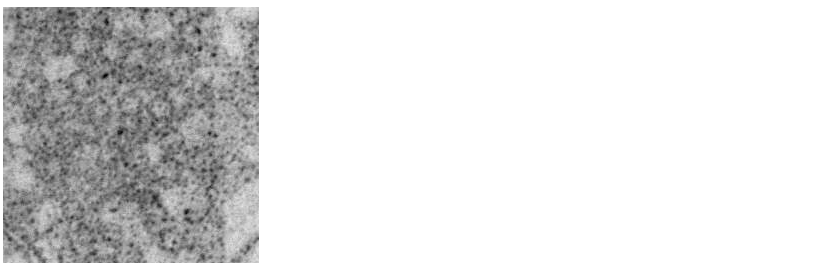
\includegraphics[scale=0.35]{img/afstand/3.png}
\end{figure}
\end{frame}

\begin{frame}
\frametitle{Segmentering med eksempelbilleder}
\begin{figure}[H]
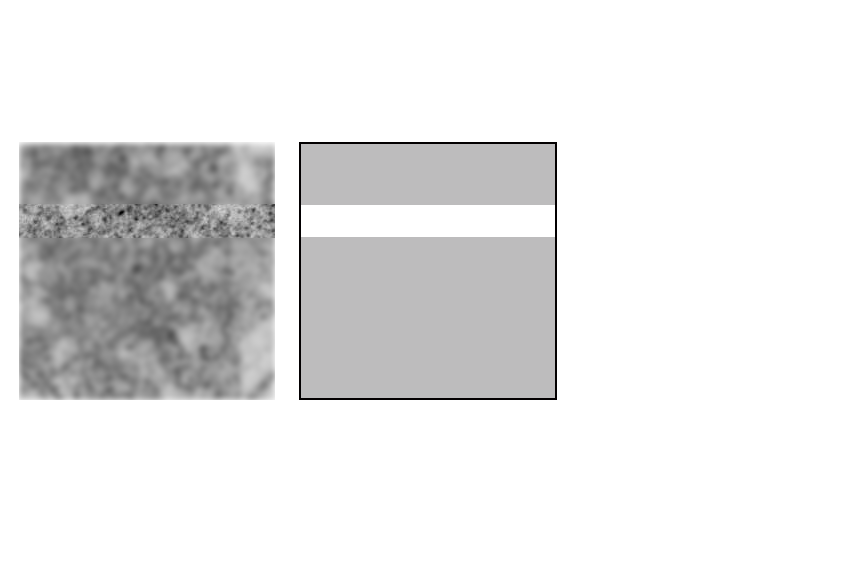
\includegraphics[scale=0.35]{img/afstand/4.png}
\end{figure}
\end{frame}

\begin{frame}
\frametitle{Segmentering med eksempelbilleder}
\begin{figure}[H]
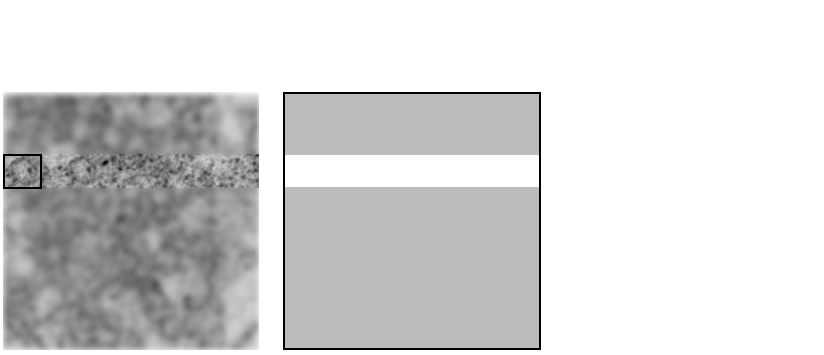
\includegraphics[scale=0.35]{img/afstand/5.png}
\end{figure}
\end{frame}


\begin{frame}
\frametitle{Segmentering med eksempelbilleder}
\begin{figure}[H]
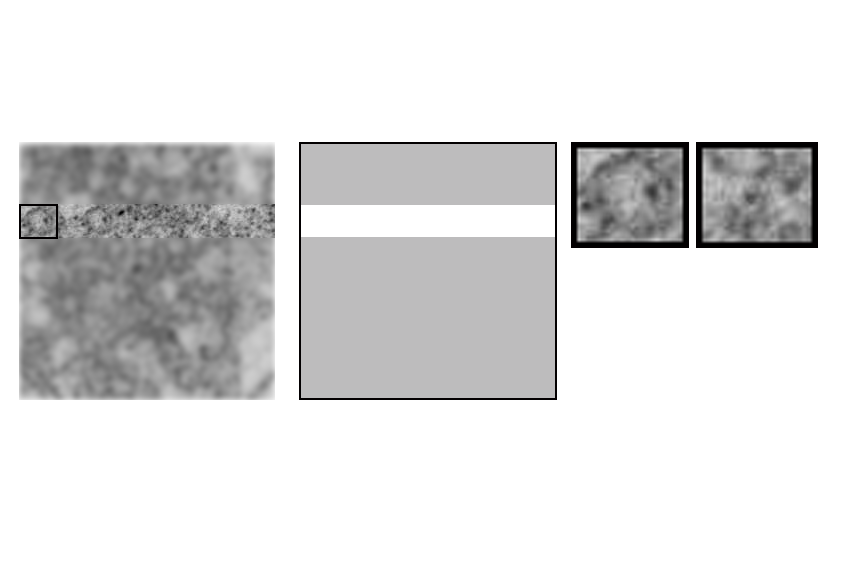
\includegraphics[scale=0.35]{img/afstand/6.png}
\end{figure}
\end{frame}


\begin{frame}
\frametitle{Segmentering med eksempelbilleder}
\begin{figure}[H]
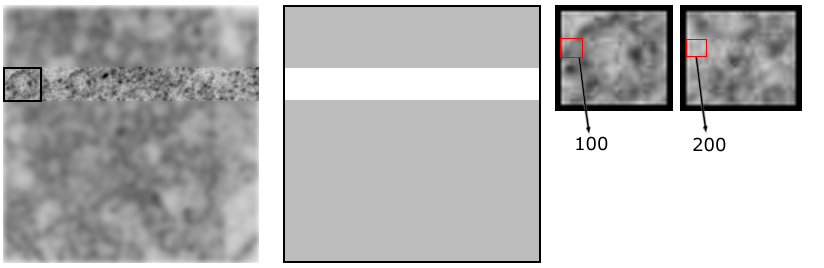
\includegraphics[scale=0.35]{img/afstand/7.png}
\end{figure}
\end{frame}


\begin{frame}
\frametitle{Segmentering med eksempelbilleder}
\begin{figure}[H]
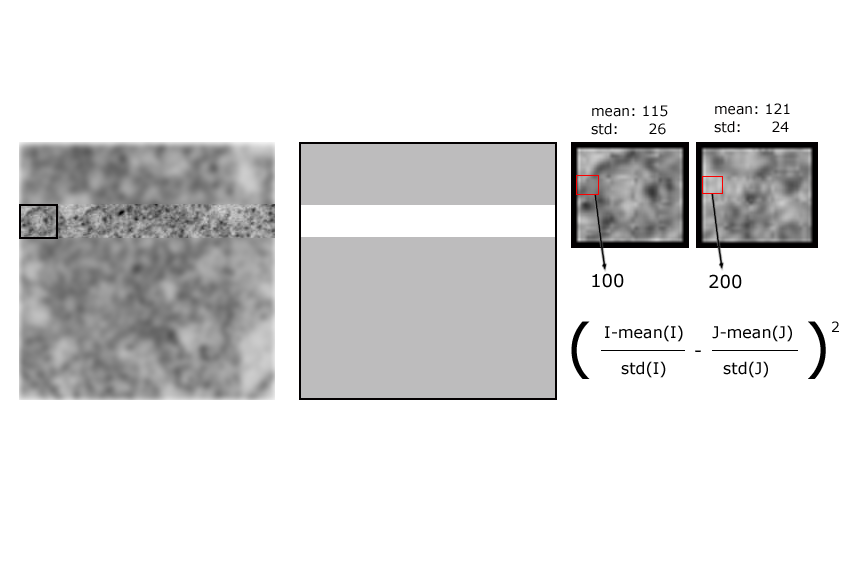
\includegraphics[scale=0.35]{img/afstand/8.png}
\end{figure}
\end{frame}

\begin{frame}
\frametitle{Segmentering med eksempelbilleder}
\begin{figure}[H]
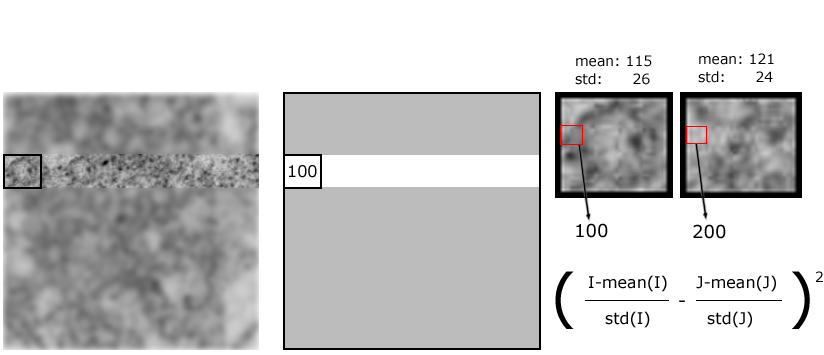
\includegraphics[scale=0.35]{img/afstand/9.png}
\end{figure}
\end{frame}

\begin{frame}
\frametitle{Segmentering med eksempelbilleder}
\begin{figure}[H]
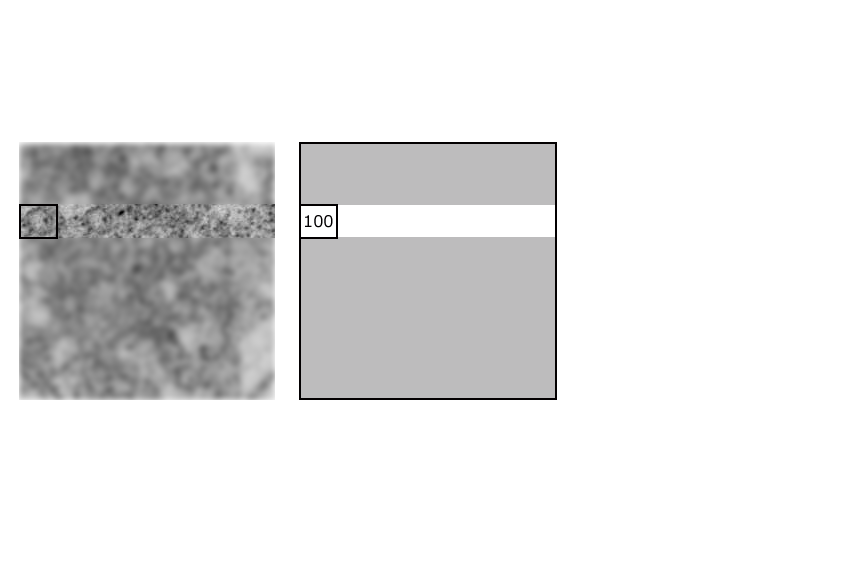
\includegraphics[scale=0.35]{img/afstand/10.png}
\end{figure}
\end{frame}

\begin{frame}
\frametitle{Segmentering med eksempelbilleder}
\begin{figure}[H]
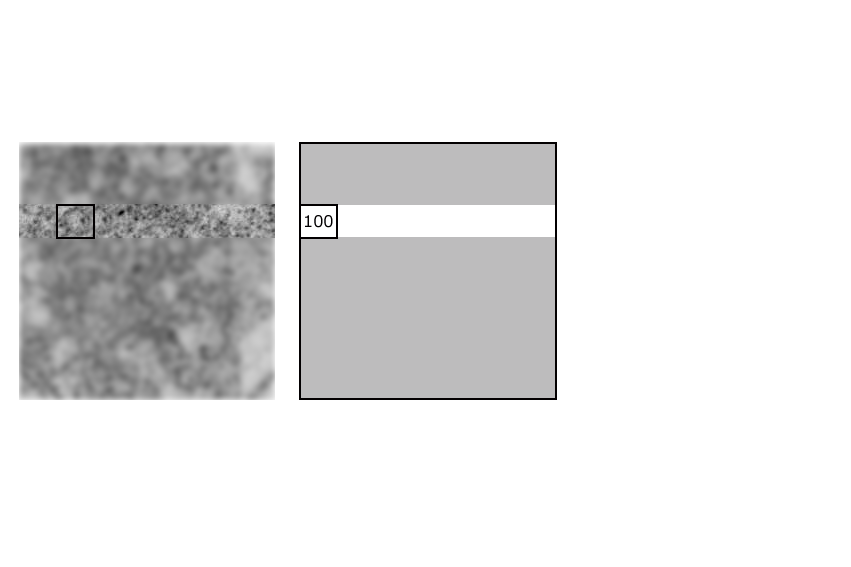
\includegraphics[scale=0.35]{img/afstand/11.png}
\end{figure}
\end{frame}

\begin{frame}
\frametitle{Segmentering med eksempelbilleder}
\begin{figure}[H]
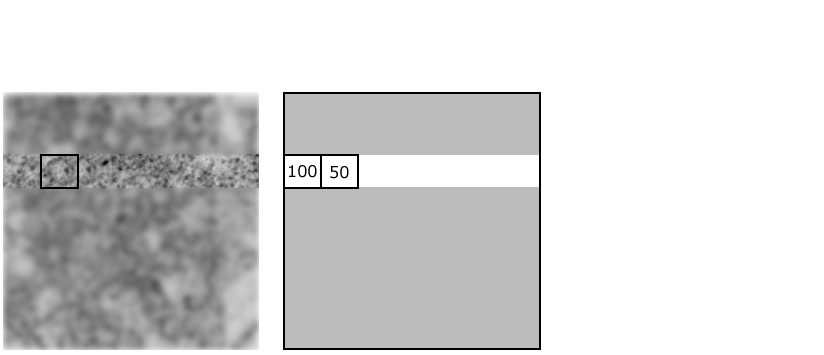
\includegraphics[scale=0.35]{img/afstand/12.png}
\end{figure}
\end{frame}

\begin{frame}
\frametitle{Segmentering med eksempelbilleder}
\begin{figure}[H]
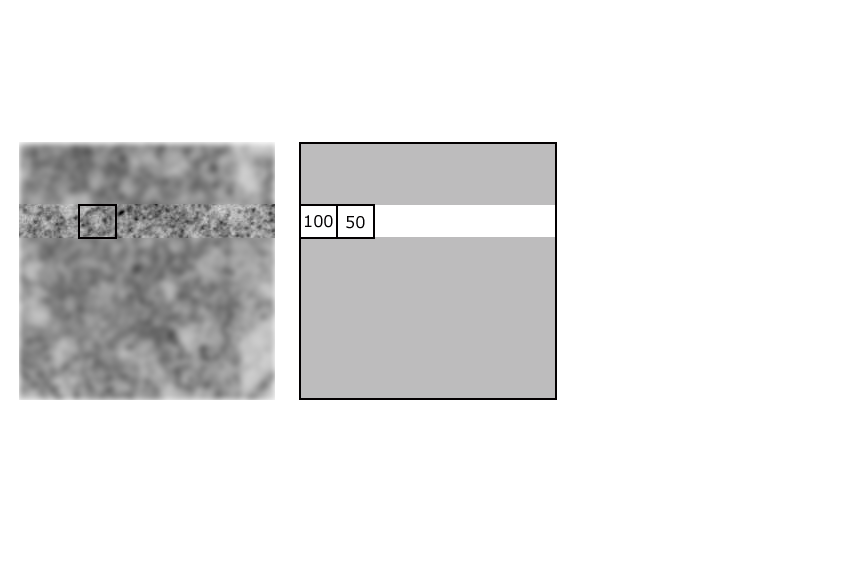
\includegraphics[scale=0.35]{img/afstand/13.png}
\end{figure}
\end{frame}

\begin{frame}
\frametitle{Segmentering med eksempelbilleder}
\begin{figure}[H]
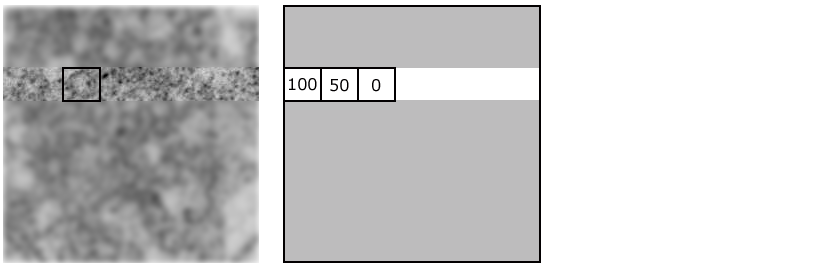
\includegraphics[scale=0.35]{img/afstand/14.png}
\end{figure}
\end{frame}


\begin{frame}
\frametitle{Segmentering med eksempelbilleder}
\begin{figure}[H]
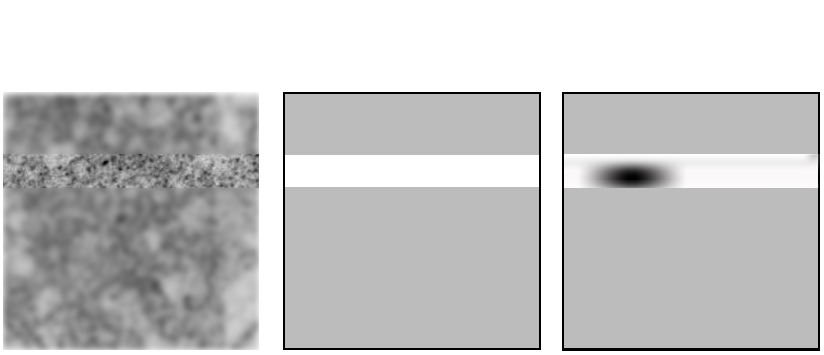
\includegraphics[scale=0.35]{img/afstand/15.png}
\end{figure}
\end{frame}

\begin{frame}
\frametitle{Segmentering med eksempelbilleder}
\begin{figure}[H]
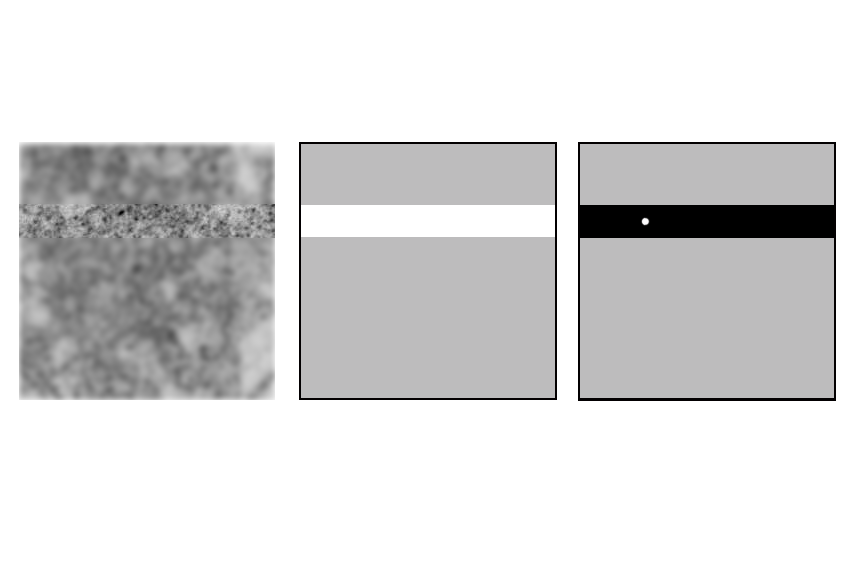
\includegraphics[scale=0.35]{img/afstand/16.png}
\end{figure}
\end{frame}

%ET kvarters præs, et kvarters disk
%Indledning krop afslutning. 
%Hav resultat på første slide
%Elevator speach
%Og så igang igen.


%Seperabel
%Foldning fungerer.

\begin{frame}
\frametitle{Resultater}
\begin{figure}[H]
	\centering
	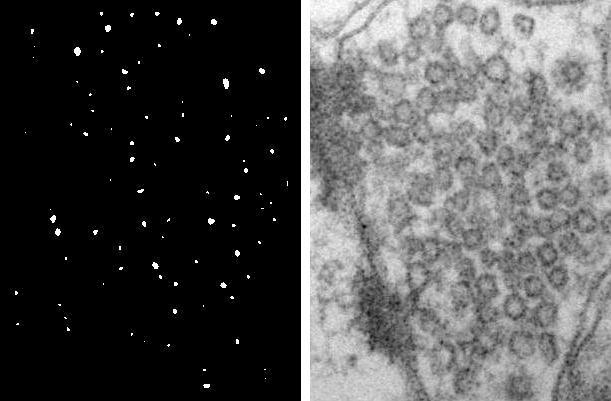
\includegraphics[scale=0.4]{img/finalmethod/thres_plot_before.png}
\end{figure}
\end{frame}

\begin{frame}
\frametitle{Resultater}
\begin{figure}[H]
	\centering
	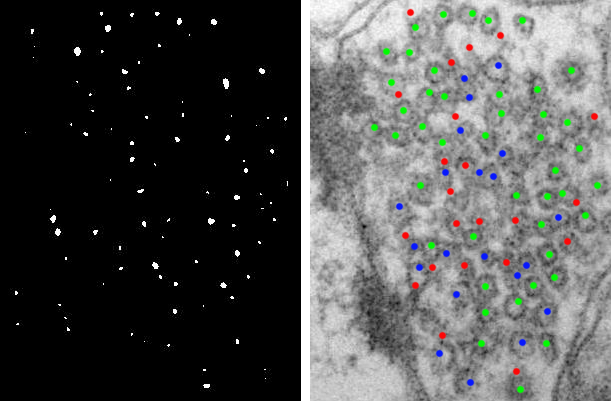
\includegraphics[scale=0.4]{img/finalmethod/thres_plot.png}
\end{figure}
\end{frame}


\begin{frame}
\frametitle{Resultater}
\begin{figure}[H]
	\centering
	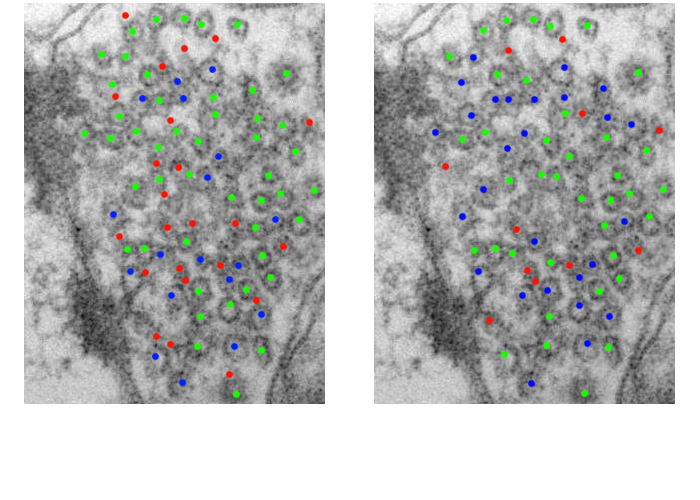
\includegraphics[scale=0.4]{img/afstand/res_1.png}
\end{figure}
\end{frame}

\begin{frame}
\frametitle{Resultater}
\begin{figure}[H]
	\centering
	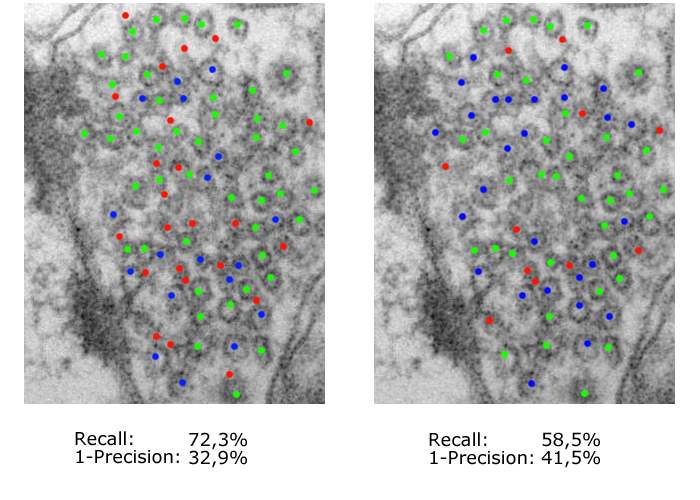
\includegraphics[scale=0.4]{img/afstand/res_2.png}
\end{figure}
\end{frame}

%Ves i et slide. med 1 og 2 <-- sensitivity (RECALL OG 1-PRES) 
%Tal i et slide
%Kombineret res af 1-2 <--- MED RECALL OG 1-PRESS.
%TAL perspektiveret til tidligere tal??

\begin{frame}
\frametitle{Resultater}

\begin{table}[H]
	\begin{tabular}{l|l|l|l}
		$\#$ ves. & Billeder & Recall & 1-Precision \\\hline
		\textbf{2}	&	\textbf{1:(a)+(b)}	 							&\textbf{0.785} 	&\textbf{0.338}\\\hline
		2	&	1:(c)+(d)	 							&0.785 	&0.414\\\hline
		2	&	1:(e)+(f)								&0.938 	&0.408\\\hline
		2	&	2:(a)+(b)  					&1 		&0.525\\\hline
		2	&	2:(c)+(d)  					&0.821 	&0.378\\\hline
		2	&	2:(e)+(f)  					&1 		&0.417\\\hline
		3	&	1:(a)+(b)+(c)	 						&0.923 	&0.4\\\hline
		3	&	1:(d)+(e)+(f)	 						&0.938 	&0.5\\\hline
		3	&	2:(a)+(b)+(c)				&1 		&0.578\\\hline
		3	&	2:(d)+(e)+(f)				&1 		&0.481\\\hline
		\textbf{4}	&	\textbf{1:(a)+(b)+(c)+(d)}						&\textbf{0.954} 	&\textbf{0.456}\\\hline
		4	&	2:(a)+(b)+(c)+(d)  			&1 		&0.582\\
	\end{tabular}
\end{table}
\end{frame}

\begin{frame}
\frametitle{Resultater}
\begin{figure}[H]
	\centering
	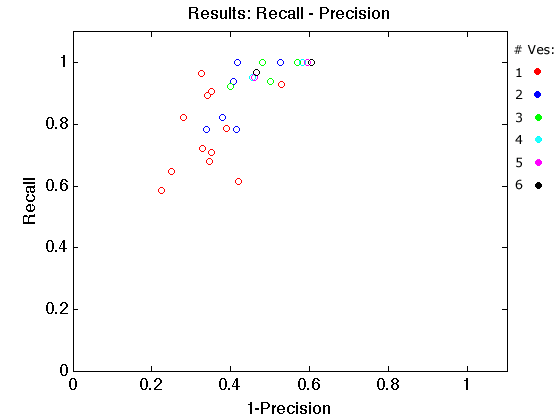
\includegraphics[scale=0.6]{img/finalmethod/recallvsprecision2.png}
\end{figure}
\end{frame}

\begin{frame}
\frametitle{Resultater}
\begin{figure}[H]
	\centering
	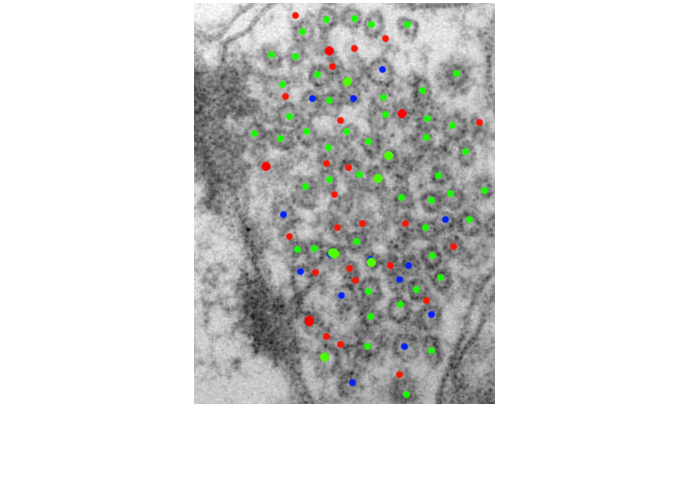
\includegraphics[scale=0.4]{img/afstand/res_3.png}
\end{figure}
\end{frame}

\begin{frame}
\frametitle{Resultater}
\begin{figure}[H]
	\centering
	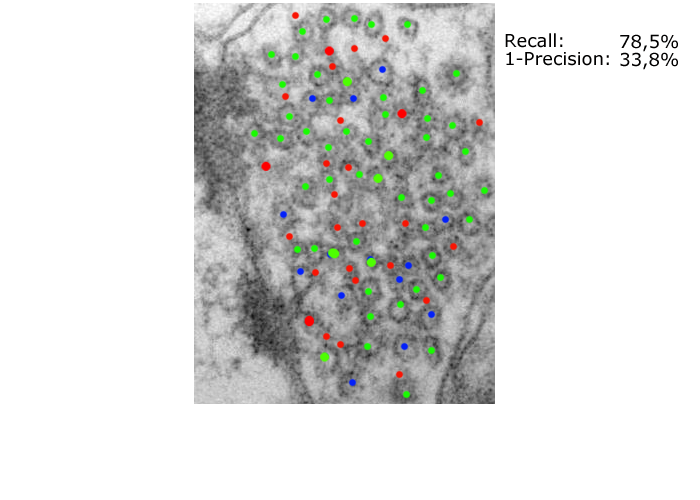
\includegraphics[scale=0.4]{img/afstand/res_4.png}
\end{figure}
\end{frame}

\begin{frame}
\frametitle{Resultater}
\begin{figure}[H]
	\centering
	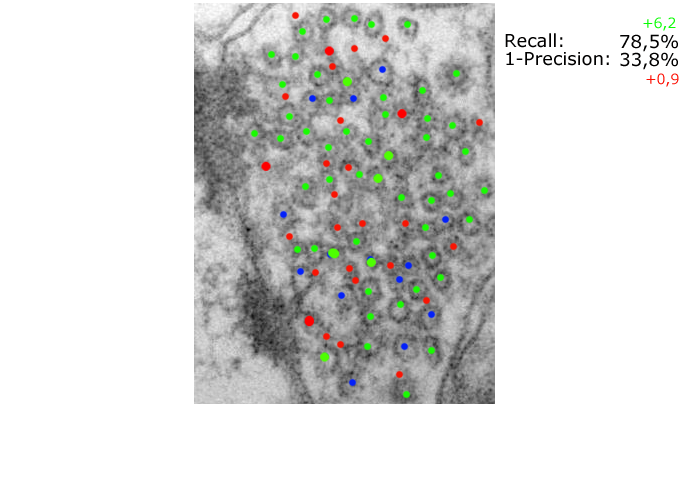
\includegraphics[scale=0.4]{img/afstand/res_5.png}
\end{figure}
\end{frame}

\begin{frame}
\frametitle{Tak}
\end{frame}

\end{document}
